\documentclass{article}

\usepackage{fancyhdr}
\usepackage{extramarks}
\usepackage{amsmath}
\usepackage{amsthm}
\usepackage{amsfonts}
\usepackage{tikz}
\usepackage[plain]{algorithm}
\usepackage{algpseudocode}
\usepackage{circuitikz}
\usepackage{booktabs}
\usepackage{graphicx}
\usepackage{gensymb}
\usepackage{hyperref}
\usepackage[all]{hypcap}
\usetikzlibrary{automata,positioning}

\hypersetup{
    colorlinks=true,
    linkcolor= blue,
    filecolor=magenta,      
    urlcolor=blue,
    pdftitle={A0276754N-LabReport},
    pdfpagemode=FullScreen,
    }

%¨¨¨¨
% Basic Document Settings
%

\topmargin=-0.45in
\evensidemargin=0in
\oddsidemargin=0in
\textwidth=6.5in
\textheight=9.0in
\headsep=0.25in

\linespread{1.1}

\pagestyle{fancy}
\lhead{Bensland}
\chead{\hmwkClass\  \hmwkTitle}
\rhead{\firstxmark}
\lfoot{\lastxmark}
\cfoot{\thepage}

\renewcommand\headrulewidth{0.4pt}
\renewcommand\footrulewidth{0.4pt}

\setlength\parindent{0pt}

%
% Create Problem Sections
%\toprule[1pt]
%\midrule[3pt]
%\bottomrule[5pt]
%

\newcommand{\enterProblemHeader}[1]{
    \nobreak\extramarks{}{Section \arabic{#1} continued on next page\ldots}\nobreak{}
    \nobreak\extramarks{Section \arabic{#1} (continued)}{Section \arabic{#1} continued on next page\ldots}\nobreak{}
}

\newcommand{\exitProblemHeader}[1]{
    \nobreak\extramarks{Section \arabic{#1} (continued)}{Section \arabic{#1} continued on next page\ldots}\nobreak{}
    \stepcounter{#1}
    \nobreak\extramarks{Section \arabic{#1}}{}\nobreak{}
}

\setcounter{secnumdepth}{0}
\newcounter{partCounter}
\newcounter{homeworkProblemCounter}
\setcounter{homeworkProblemCounter}{1}
\nobreak\extramarks{Section \arabic{homeworkProblemCounter}}{}\nobreak{}

%
% Homework Problem Environment
%
% This environment takes an optional argument. When given, it will adjust the
% problem counter. This is useful for when the problems given for your
% assignment aren't sequential. See the last 3 problems of this template for an
% example.
%
\newenvironment{homeworkProblem}[1][-1]{
    \ifnum#1>0
        \setcounter{homeworkProblemCounter}{#1}
    \fi
    \section{Section \arabic{homeworkProblemCounter}}
    \setcounter{partCounter}{1}
    \enterProblemHeader{homeworkProblemCounter}
}{
    \exitProblemHeader{homeworkProblemCounter}
}

%
% Homework Details
%   - Title
%   - Due date
%   - Class
%   - Section/Time
%   - Instructor
%   - Author
%

\newcommand{\hmwkTitle}{Lab Report}
\newcommand{\hmwkDueDate}{November 03, 2023}
\newcommand{\hmwkClass}{Electrical Energy Systems}
\newcommand{\hmwkClassInstructor}{National University of Singapore EE2022}
\newcommand{\hmwkAuthorName}{\textbf{Karl Alexander Bensland} \and \textbf{A0276754N}}

%
% Title Page
%

\title{
    \vspace{2in}
    \textmd{\textbf{\hmwkClass:\ \hmwkTitle}}\\
    \normalsize\vspace{0.1in}\small{Due\ on\ \hmwkDueDate}\\
}

\author{\hmwkAuthorName}
\date{}

\renewcommand{\part}[1]{\textbf{\large Part \Alph{partCounter}}\stepcounter{partCounter}\\}

%
% Various Helper Commands
%

% Useful for algorithms
\newcommand{\alg}[1]{\textsc{\bfseries \footnotesize #1}}

% For derivatives
\newcommand{\deriv}[1]{\frac{\mathrm{d}}{\mathrm{d}x} (#1)}

% For partial derivatives
\newcommand{\pderiv}[2]{\frac{\partial}{\partial #1} (#2)}

% Integral dx
\newcommand{\dx}{\mathrm{d}x}

% Alias for the Solution section header
\newcommand{\solution}{\textbf{\large Solution}}

% Probability commands: Expectation, Variance, Covariance, Bias
\newcommand{\E}{\mathrm{E}}
\newcommand{\Var}{\mathrm{Var}}
\newcommand{\Cov}{\mathrm{Cov}}
\newcommand{\Bias}{\mathrm{Bias}}

\begin{document}

\maketitle

\pagebreak

\tableofcontents

\pagebreak

    \subsection{Introduction}
    The report starts by exploring the fundamental elements of AC power measurement, focusing specifically on an R-L load. Here, we measure and analyze various parameters like voltage, current, real power, and reactive power. Building on this foundation, the report delves into the concept of power factor — explaining why it's critical and outlining practical ways to improve it using capacitors.\\
    Transitioning from power metrics, the report shifts its focus to transformers, key components in the electrical power distribution landscape. Through short-circuit and open-circuit tests on two types of transformers, we determine their equivalent circuit parameters. These insights allow us to better understand the operational efficiency and characteristics of transformers in a real-world setting.\\
    As a natural extension of this, the report then covers the topic of power loss in transmission lines. This is a key concern in electrical engineering, and we approach it through experiments carried out in two different settings—one without transformers and another incorporating them. By examining parameters like line current, power, and reactive power, we provide a understanding of how much energy is lost during transmission and under what conditions.\\
    The findings in this report are complemented by data from the PLECS simulation tool. This allows us to conduct a detailed comparison between theoretical concepts and practical measurements, helping to identify and discuss any discrepancies.\\
    In terms of the AC values used in this report, it's important to note that they are represented as peak values. For those who are interested in RMS or average values, these can be calculated by dividing the peak values by $\sqrt{2}$.\\
    To round out the discussion, \hyperref[subsec:erors]{Section 4} of the report will specifically address potential errors that could have influenced the experiments and suggestions for improvement. Additionally, this report discusses tangible benefits of optimizing power factor and the strategic use of transformers in electrical power systems.
        
    \pagebreak

\begin{homeworkProblem}


    
    \subsection{AC Power for an R-L Load}

    
    \begin{figure}[h]
    \centering
    \begin{circuitikz}
        \draw (0,4) 
        to[sV, v={$V_s$}] (0,0); 
        \draw (0,4) -- (2,4)
        to[R, l={$1.2\Omega$}, *-*] (4,4)
        to[L, l={$2.2mH$}, *-*] (6,4);
        \draw (6,4) -- (8,4);
        \draw (6,0) -- (8,0);
        \draw (9.5,4)
        to[R, l={$16\Omega$}, *-*] (9.5,2)
        to[L, l={$90mH$}, v={$V_L$}, *-*] (9.5,0);
        \draw (8,4) -- (9.5,4);
        \draw (8,0) -- (9.5,0);
        \draw[->] (0.5,3.8) -- (1.5,3.8) node[midway, anchor=north] {$I_s$};
        \draw[->] (6.5,3.8) -- (7.5,3.8) node[midway, anchor=north] {$I_{\text{Load}}$};
        \draw[->] (8,2.5) -- (8,1.5) node[midway, anchor=east] {$V_{\text{Load}}$};
        \draw[dashed] (8.5,4.5) -- (10.5,4.5) -- (10.5,-0.5) -- (8.5,-0.5) -- cycle;
        \draw (0,0) -- (6,0);
        \node at (9.5,-1) {R-L Load};
        \node at (4,3.5) {Transmission line};
        
    \end{circuitikz}
    \caption{R-L Load}
    \label{fig:rl_load}
    \end{figure}  

    \begin{table}[H]
       \small
       \centering
       \begin{tabular}{l|ccccccr}
       \toprule\toprule
       \textbf{} & \textbf{$V_{Source} (V)$} & \textbf{$I_{Source} (A)$} & \textbf{$P_{Source} (W)$} & \textbf{$Q_{Source} (var)$} & \textbf{$P.F.\, source$} \\
       \midrule
       \text{Measurements}&20.5&0.528&6.5&8.6&0.606\\
       \midrule
       \text{Simulation}&20.75&0.61& 6.34 & 11.0 & 0.501 \\
       \toprule\toprule
       \textbf{} & \textbf{$V_{Load} (V)$} & \textbf{$I_{Load} (A)$} & \textbf{$P_{Load} (W)$} &
       \textbf{$Q_{Load} (var)$} & \textbf{$P.F.Load$} & \textbf{$V_L (V)$} \\
       \midrule
       \text{Measurements}&20.0&0.528&6.2&8.5&0.584&16.6\\
       \midrule
       \text{Simulation}&20.0&0.616&6.16&10.7&0.501&17.4\\
       \bottomrule 
       \end{tabular}
       \caption{Measurements: AC Power for an R-L Load}
       \label{Table 1_RL}
    \end{table}

    From these measurements we can analyse the power-line losses and calculate the resistance and inductance values.
    
    \begin{align*}
    I^2 R_{Line} &= P_{Line} \\
    (0.528\, \text{A})^2 \times 1.2\, \Omega &= 0.3345\, \text{W}\\
    \end{align*}

    \begin{minipage}{.5\textwidth}
    \begin{align*}
        R_{\text{Load}} &= \frac{\sqrt{V_{Load}^2 - V_{L}^2}}{|I|}   \\
        R_{\text{Load}} &= \frac{11.1V}{0.528A}  \\
        R_{\text{Load}} &= 21.0\ohm
    \end{align*}
    \end{minipage}%
    \begin{minipage}{.5\textwidth}
    \begin{align*}
        R_{\text{Line}} &= \frac{|P_{Source}-P_{Load}|}{|I|^2}   \\
        R_{\text{Line}} &= \frac{0.3W}{(0.528A)^2}  \\
        R_{\text{Line}} &= 1.08\ohm
    \end{align*}
    \end{minipage}
 \\
    Which means we have an error of: 
    $ |\frac{R_{calculated} - R_{Ideal}}{R_{Ideal}}| \rightarrow$ $ \frac{5\ohm}{16\ohm} = 31.1\% $ \textbf{\&} $ \frac{0.120\ohm}{1.2\ohm} = 10\%$ \\

\pagebreak

 \[
    V = j\omega L \cdot I
 \]

    \begin{minipage}{.5\textwidth}
    \begin{align*}
        L_{\text{Load}} &= \frac{|V_L|}{|I|\times 2\pi \times 50\, \text{Hz}}   \\
        L_{\text{Load}} &= \frac{16.6V}{0.528A\times 2\pi \times 50\, \text{Hz}}  \\
        L_{\text{Load}} &= 0.10007\, \text{H} \approx 100mH
    \end{align*}
    \end{minipage}%
    \begin{minipage}{.5\textwidth}
    \begin{align*}
        L_{\text{Line}} &= \frac{|Q_{Source}|- |Q_{Load}|}{|I|^2\times 2\pi \times 50\, \text{Hz}}   \\
        L_{\text{Line}} &= \frac{0.1var}{(0.528A)^2\times 2\pi \times 50\, \text{Hz}}  \\
        L_{\text{Line}} &= 0.00114178\, \text{H} \approx 1.14mH
    \end{align*}
    \end{minipage}

    Which means we have an error of: 
    $ |\frac{L_{calculated} - L_{Ideal}}{L_{Ideal}}| \rightarrow \frac{10mH}{90mH} = 11.1\% $ \textbf{\&} $ \frac{1.06mH}{2.2mH} = 48\%$ \\

    \begin{figure}[ht]
        \centering
        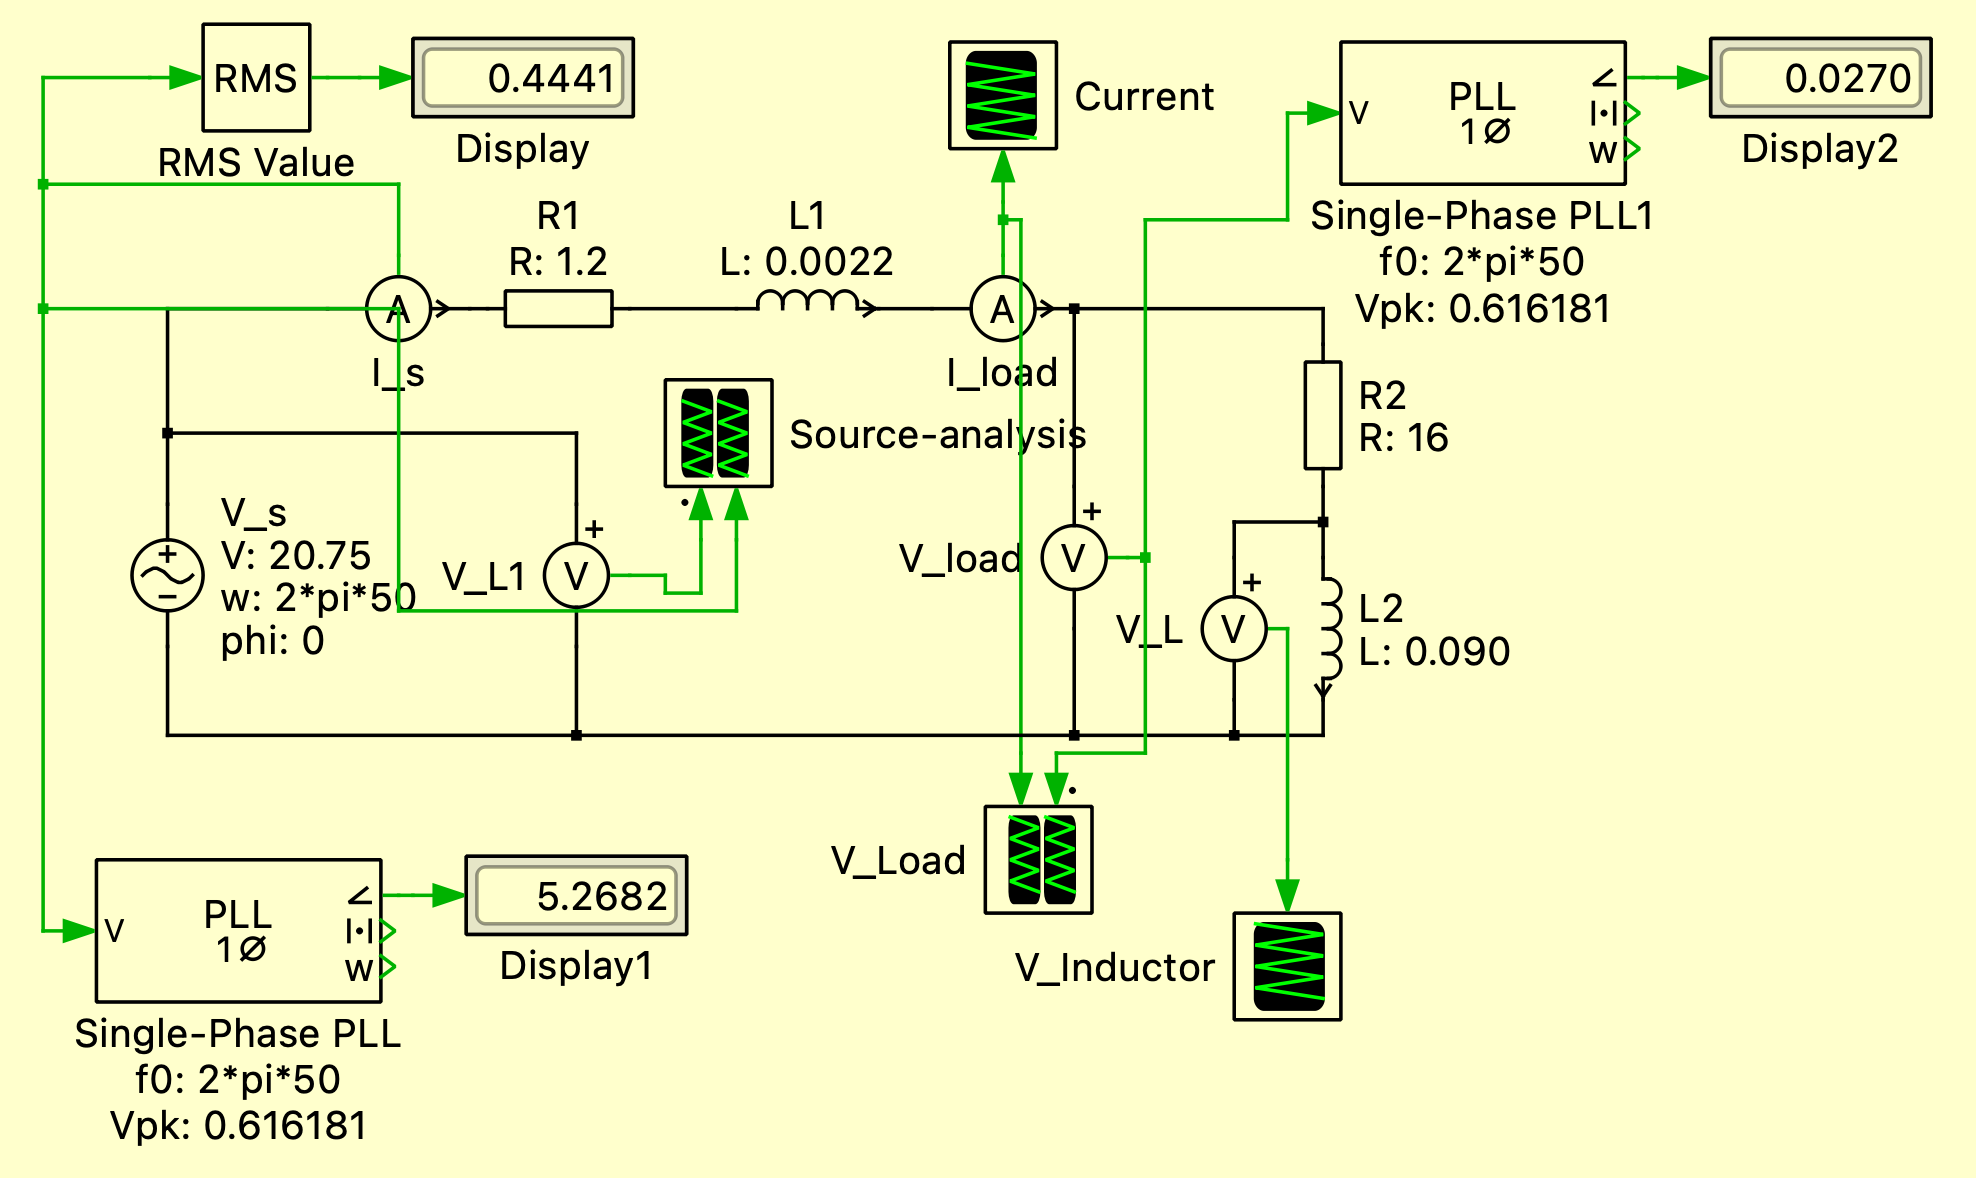
\includegraphics[width=0.5\linewidth]{images/Sim.1.png}
        \caption{Simulation of Circuit Fig.\ref{fig:rl_load}}
        \label{fig:Sim.1}
    \end{figure}

    An 11.1\% discrepancy is significant, warranting further verification. To cross-check the accuracy of our measurements, we turned to PLECS simulations, which yielded slightly different results than our manual calculations.
    The simulated current is 0.616A, which means using $I^2*R = P$ $\rightarrow$ 
    $P_{sim} = (0.616\, \text{A})^2 \times 1.2\, \Omega \approx 0.455\, \text{W} $ \\
    Similarly, the simulated value of $|V_L| = 17.2 \rightarrow L_{sim} = \frac{17.2V}{0.616A\times 2\pi \times 50\, \text{Hz}} \approx 88.9mH$ \\
    Which gives us an error of:
    $ |1 - \frac{L_{sim}}{L_{Ideal}}| = 1 - \frac{88.9mH}{90mH} = 1.2\% $ \\
    While not perfectly aligned with our manual calculations, the simulated results are within a reasonable margin of error, suggesting that the models and calculations are generally reliable, however our measurements seem to be further away than expected. Since we did not measure the voltages over each of the components separately the main source of error probably arises from there, other possibilities are discussed in \hyperref[subsec:erors]{Section 4}. Further note that since the measurements of Q where not accurate enough, the calculated Value of $L_{Line}$ should not be considered accurate. One could re due the experiment and specifically measure the voltage over the line inductance to get a more accurate calculation.

    \pagebreak
    
    \subsection{Power Factor Improvement Using a Capacitor}\label{sub:test}

    \begin{figure}[h]
    \centering
    \begin{circuitikz}
        \draw (0,4) 
        to[sV, v={$V_s$}] (0,0); 
        \draw (0,4) -- (2,4)
        to[R, l={$1.2\Omega$}, *-*] (4,4)
        to[L, l={$2.2mH$}, *-*] (6,4);
        \draw (6,4) -- (8,4);
        \draw (6,0) -- (8,0);
        \draw (9.5,4)
        to[R, l={$16\Omega$}, *-*] (9.5,2)
        to[L, l={$90mH$}, v={$V_L$}, *-*] (9.5,0);
        \draw (8,4) -- (9.5,4);
        \draw (8,0) -- (9.5,0);
        \draw[->] (0.5,3.8) -- (1.5,3.8) node[midway, anchor=north] {$I_s$};
        \draw[->] (6.5,3.8) -- (7.5,3.8) node[midway, anchor=north] {$I_{\text{Load}}$};
        \draw[->] (7,2.5) -- (7,1.5) node[midway, anchor=east] {$V_{\text{Load}}$};
        \draw[dashed] (8.5,4.5) -- (10.5,4.5) -- (10.5,-0.5) -- (8.5,-0.5) -- cycle;
        \draw (0,0) -- (6,0);
        \node at (9.5,-1) {R-L Load};
        \node at (4,3.5) {Transmission line};
        %capacitor
        \draw (7.7,4)
        to[C, l={$C$}] (7.7,0.5)
        -- (7.7,0);
    \end{circuitikz}
    \caption{Power Factor Improvement}
    \label{fig:rlc_load}
    \end{figure}  

    Utilizing the measurements from the circuit depicted in Figure \ref{fig:rl_load}, we determined the value of capacitance needed to counterbalance the reactive power generated by the inductor.
    
    \begin{align*}
    |Q_C| &= |Q_L| = V_L * I_{L} \\
    Q_L &= \frac{V_L^2}{|Z_C|} \\
    \leftrightarrow C &= \frac{Q_L}{V_L^2*\omega} \\
    C &= \frac{8.5var}{(20V)^2*2*\pi*50Hz} \\
    C &\approx 67.6\mu F
    \end{align*}

    So after inserting a capacitance with 67.6 $\mu$ F in the circuit like in Figure \ref{fig:rlc_load} the following values where measured:
    
    \begin{table}[H]
       \small
       \centering
       \begin{tabular}{l|ccccccr}
       \toprule\toprule
       \textbf{} &\textbf{$V_{Source} (V)$} & \textbf{$I_{Source} (A)$} & \textbf{$P_{Source} (W)$} & \textbf{$Q_{Source} (var)$} & \textbf{$P.F.\, source$} \\
       \midrule
       \text{Measurements}&20.5&0.311&6.30&0.00&0.996\\
       \midrule
       \text{Simulation}&20.8&0.322&6.30&2.29&$0.940$\\
       \toprule\toprule
       \textbf{} & \textbf{$V_{Load} (V)$} & \textbf{$I_{Load} (A)$} & \textbf{$P_{Load} (W)$} &
       \textbf{$Q_{Load} (var)$} & \textbf{$P.F.Load$}\\
       \midrule
       \text{Measurements}&20.0&0.3118&6.20&0.00&0.995\\
       \midrule
       \text{Simulation}&20.4&0.322&6.17&2.24&$0.940$\\
       \bottomrule 
       \end{tabular}
       \caption{Measurements: Power Factor Improvement using Capacitor}
       \label{Table2_Capacitor}
    \end{table}

    Lets see if the power factor of the Source and Load is around 1 which guarantees that our $Q_{Source}$ and $Q_{Load}$ is around 0 and validates our measurements. To calculate the P.F. we check the angle between the Voltage and the Current:

    It's worth noting that both \( Q_{source} \) and \( Q_{load} \) register as zero, despite the fact that the capacitance is designed solely to offset the reactive power from the load, not from the transmission line. To validate the accuracy of these measurements, we cross-reference them with simulated values.
    A power factor close to 1 would corroborate that \( Q_{Source} \) and \( Q_{Load} \) are indeed approximately zero. To calculate the P.F., we assess the phase angle between the voltage and current.

    \begin{figure}[ht]
        \centering
        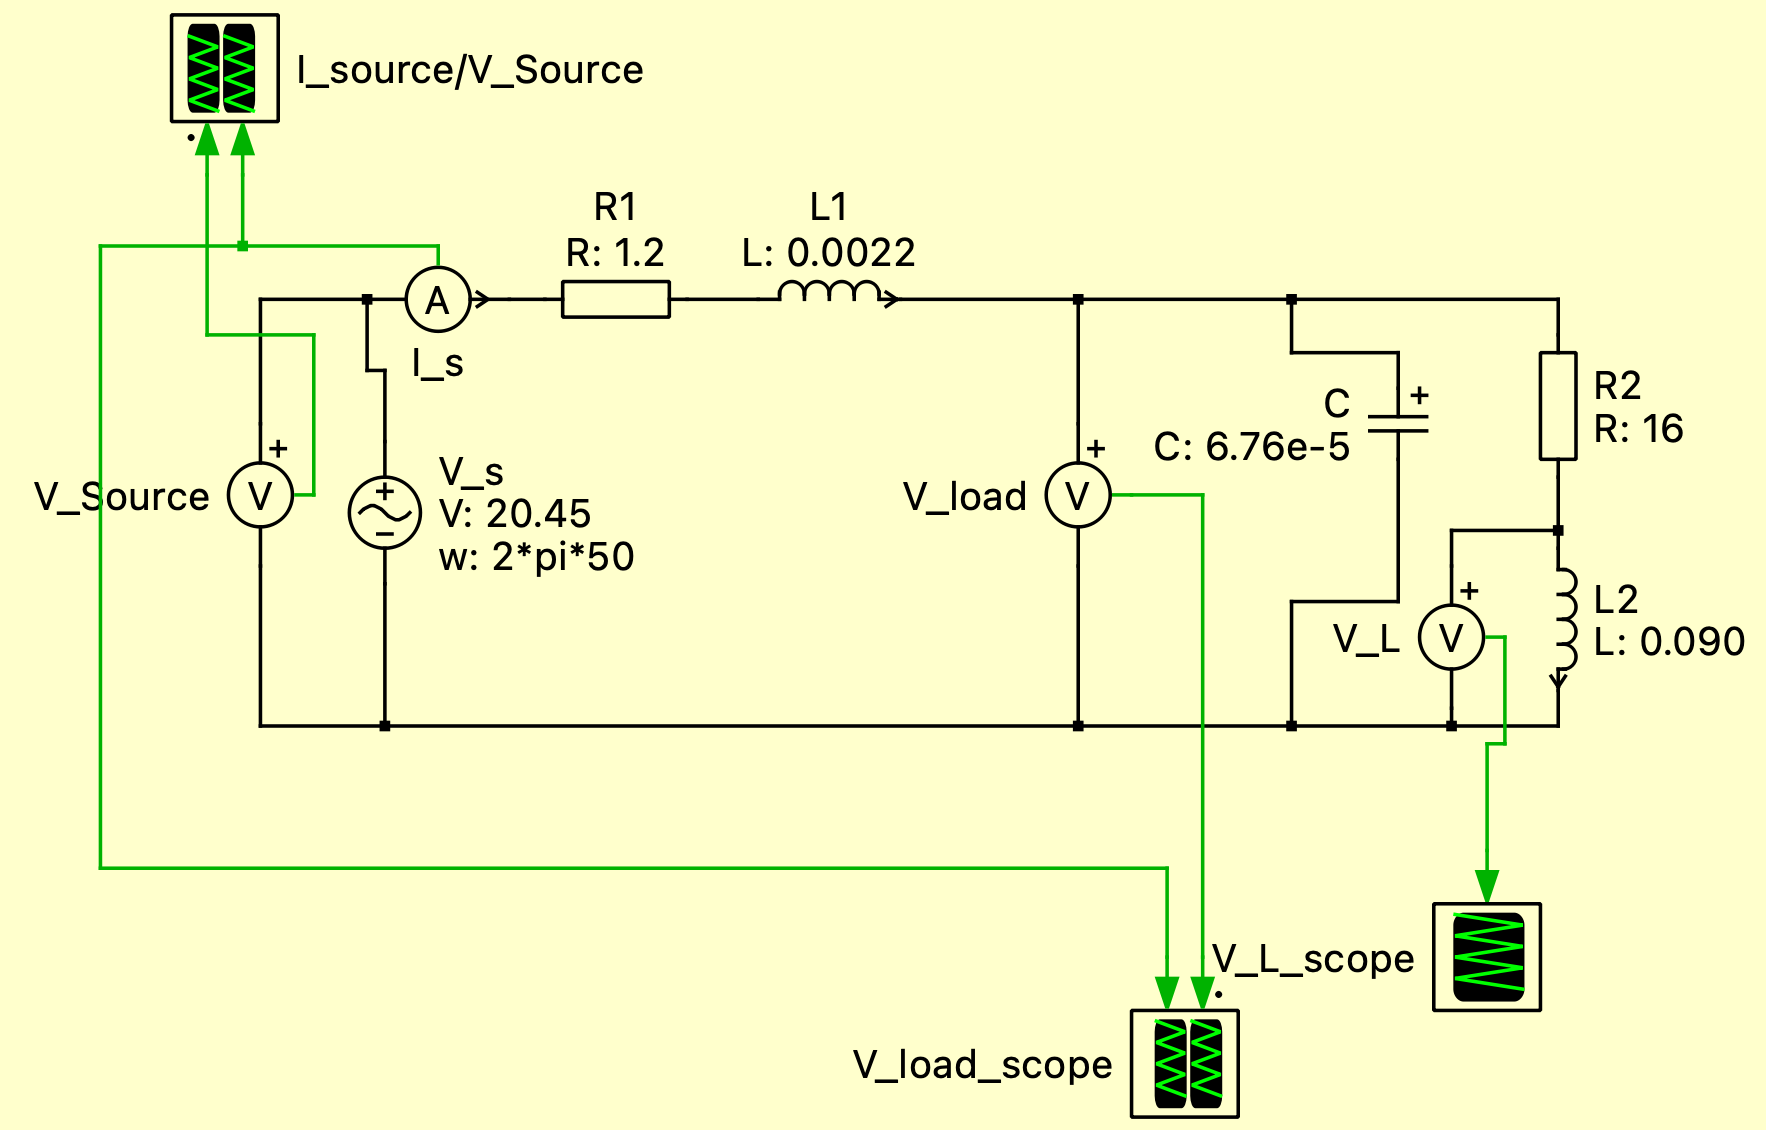
\includegraphics[width=0.6\textwidth]{images/Sim.2.png}
        \caption{Simulation of Circuit \ref{fig:rlc_load}}
        \label{fig:SimulationCircuit2}
    \end{figure}

    \begin{figure}[ht]
      \centering
      \begin{minipage}{0.5\textwidth}
        \centering
        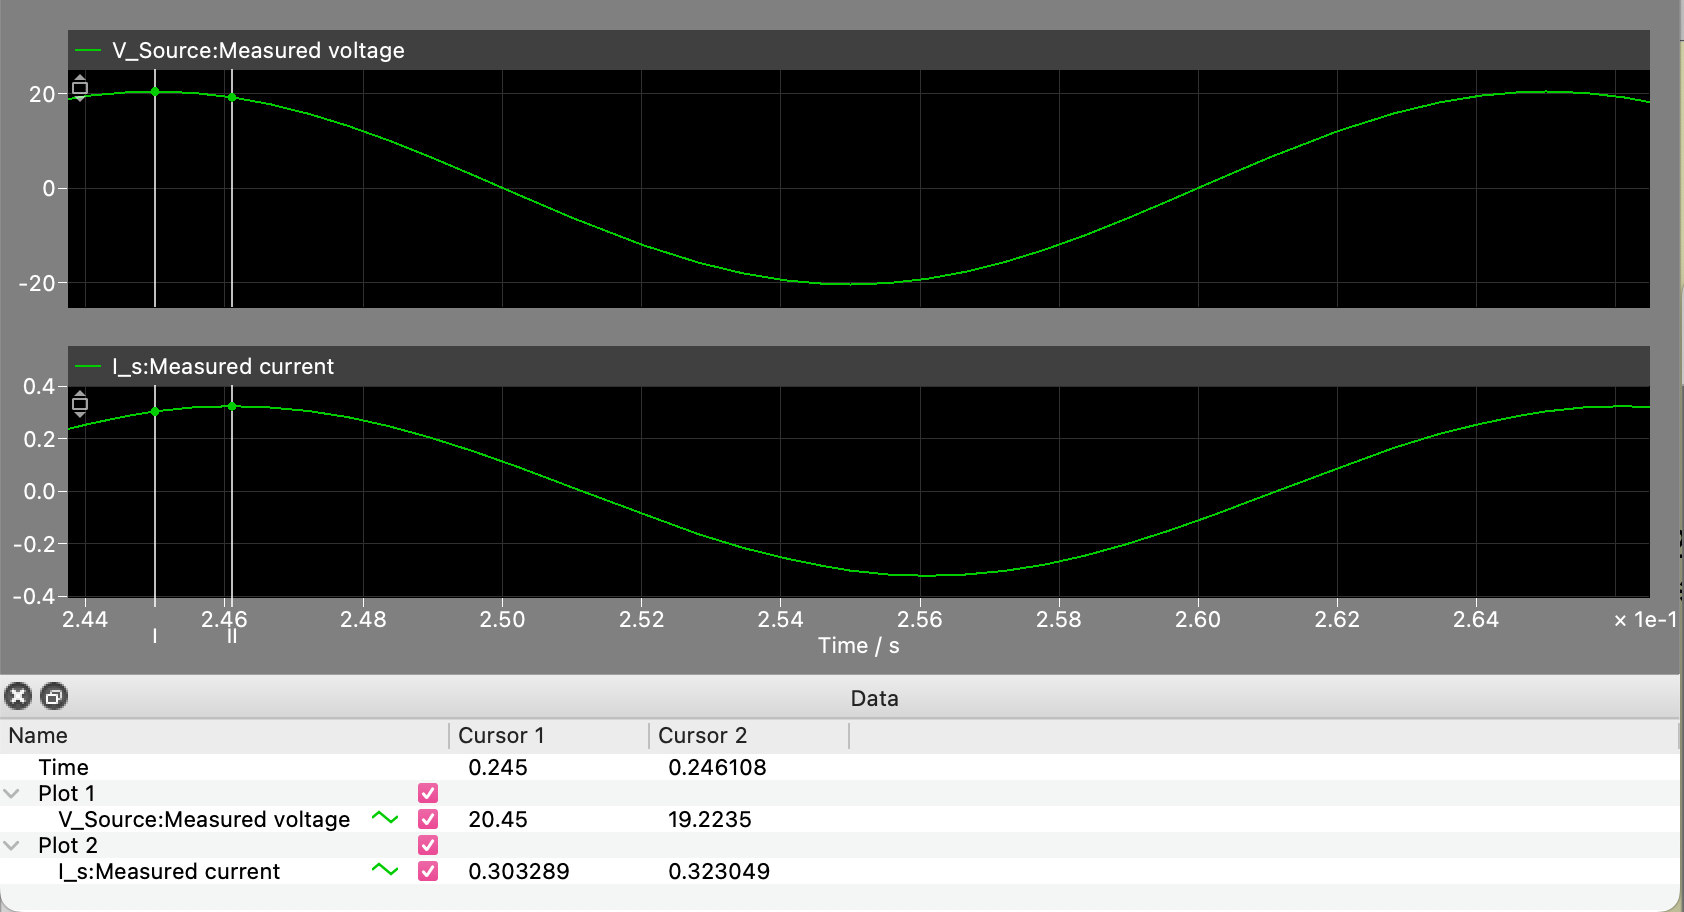
\includegraphics[width=0.95\linewidth]{images/PhaseSource_Sim2.png}
        \caption{Sim: Top;$V_{Source}$ Bottom;$I_{Source}$}
        \label{fig:PhaseSource}
      \end{minipage}%
      \hfill
      \begin{minipage}{0.5\textwidth}
        \centering
        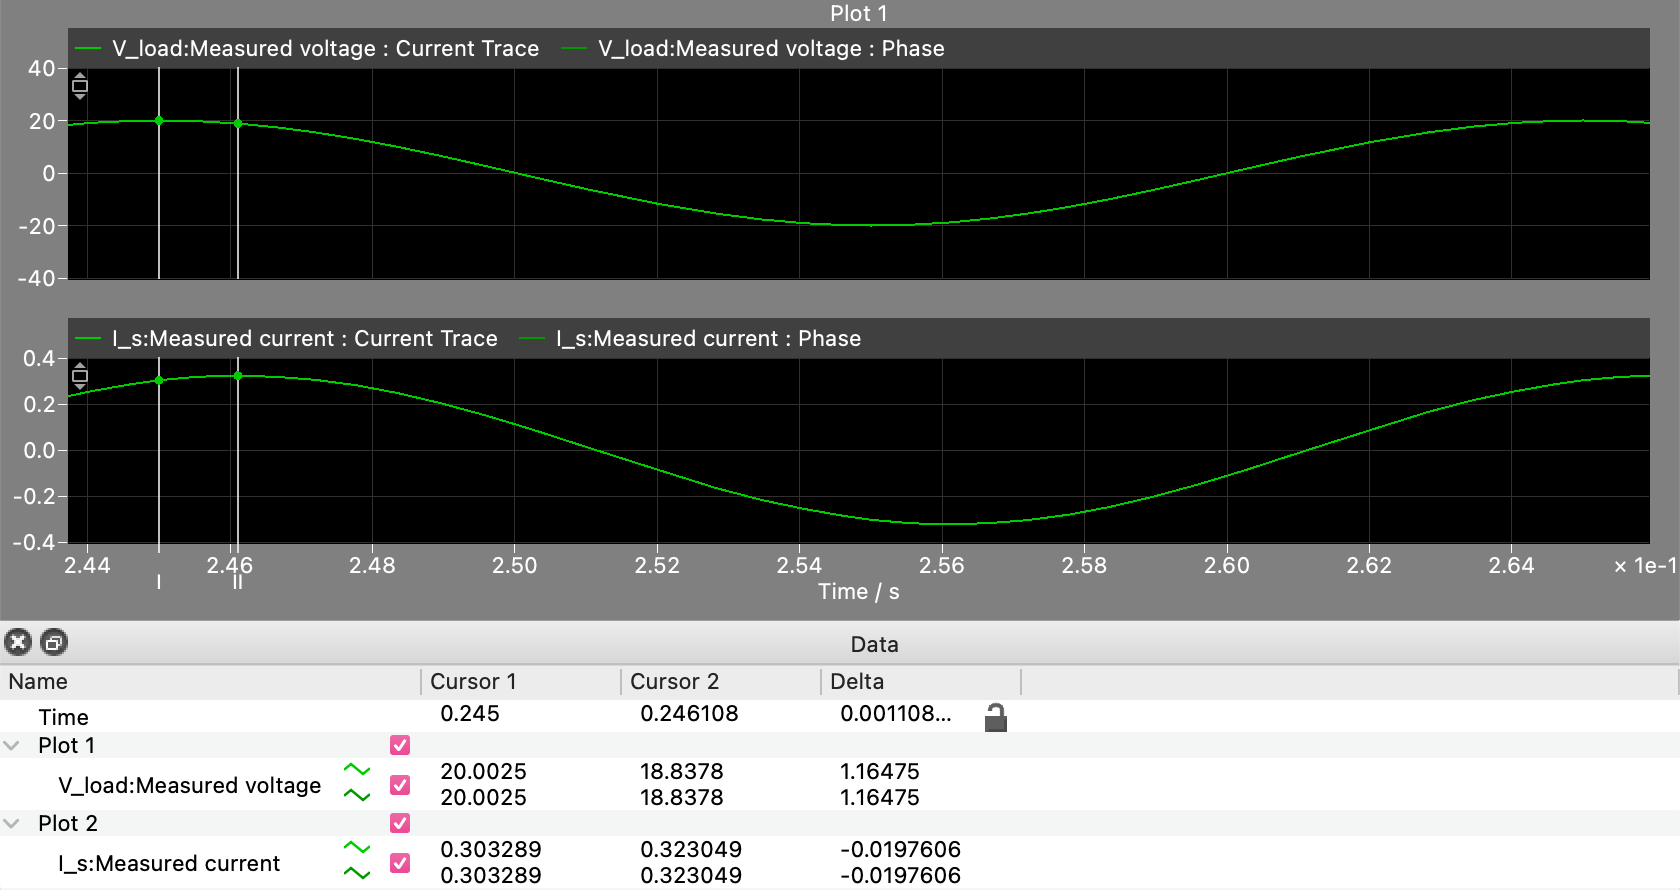
\includegraphics[width=0.97\linewidth]{images/PhaseLoad_Sim2.png}
        \caption{Sim: Top;$V_{Load}$ Bottom;$I_{Load}$}
        \label{fig:PhaseLoad}
      \end{minipage}
    \end{figure}

    In analyzing the power factor from the simulation, our primary objective is to confirm that both the source and the load have identical power factors. We do this by measuring the time delta between the voltage and current peaks. In the simulation, both the source and load exhibit a delta of 1.11 ms. Given that both operate at 50 Hz, the similarity in time deltas verifies that our measurements are consistent with the simulation. To further validate our results, we can explicitly calculate the power factor as follows:
    
    \[
    P.F._{sim.Source} = P.F._{sim.Load} = cos( \frac {\delta t}{T}*360 \degree )
    = cos(\frac{0.111ms}{20ms}*360 \degree ) = cos(20.0 \degree ) = 0.940\\
    \]
    Which shows us that our measurements are reasonable and that the inductive Load of the Transmission Line only plays a minor role in the beahviour of our system.\\
    \\
    With the compensating capacitance in place, the reactive power is significantly reduced. This allows more power to be effectively transferred to the load instead of being wasted as losses due to inductance. It's worth noting that our measured values showed a P.F. of 0.995, implying a phase angle close to 5 degrees. However, the measured reactive power (\( Q \)) was approximately zero VAR, which seems contradictory. For Figure \ref{fig:power_triangles}, we assumed \( Q = 0 \), but adopting the power factor value of 0.995 would result in \( Q = 0.62 \) VAR. While not a massive difference, this discrepancy falls within the realm of measurement error, a topic further explored in the \hyperref[subsec:erors]{Errors} subsection.
    
    \begin{figure}[ht]
        \centering
        \begin{tikzpicture}[scale=0.54, transform shape]
        
        % Drawing the first triangle
        \draw[thick,->] (0,0) -- (6.5,0) node[midway,below] {\( P_{\text{source}} = 6.5 \)W};
        \draw[thick,->] (6.5,0) -- (6.5,8.6) node[midway,right] {\( Q_{\text{source}} = 8.6 \)var};
        \draw[thick,->] (0,0) -- (6.5,8.6);
        
        % Angle for the first triangle
        \draw (2,0) arc (0:53.5:2) node[midway, right] {\( \theta = 52.9 \degree \)};
        \draw (3, 4.25) node[right] {\( S_{Source} = 10.8VA \)};
        
        % Offset for the second triangle (x-offset is 8 units)
        \newcommand{\xoffset}{8}
        
        % Drawing the second triangle
        \draw[thick,->] (\xoffset,0) -- (\xoffset+6.3,0) node[midway,below] {\( P_{\text{source}}' = 6.3\)W};
        \draw[thick,->] (\xoffset+6.3,0) -- (\xoffset+6.3,0.02) node[midway,right] {\( Q' = 0var\)};
        \draw[thick,->] (\xoffset,0) -- (\xoffset+6.3,0.02);
        
        % Angle for the second triangle
        %\draw (\xoffset+2,0) arc (0:53.5:2) node[midway, right] {\( \theta' \)};
        \draw (\xoffset+3, 0.25) node[right] {\( S_{Source}' = 6.3VA \)};
        
        \end{tikzpicture}
        \caption{Power Triangles: Left; \hyperref[fig:rl_load]{ \(RL_{Source}\) } Right; \hyperref[fig:rlc_load]{ \(RLC_{Source}\) }}
        \label{fig:power_triangles_source}
    \end{figure}
    
    
    \begin{figure}[ht]
    \centering
    \begin{tikzpicture}[scale=0.50, transform shape]
    
    % Drawing the first triangle
    \draw[thick,->] (0,0) -- (6.2,0) node[midway,below] {\( P_{\text{load}} = 6.2 \)W};
    \draw[thick,->] (6.2,0) -- (6.2,8.5) node[midway,right] {\( Q_{\text{load}} = 8.5 \)var};
    \draw[thick,->] (0,0) -- (6.2,8.5);
    
    % Angle for the first triangle
    \draw (2,0) arc (0:53.5:2) node[midway, right] {\( \theta = 53.9 \degree \)};
    \draw (3, 4.25) node[right] {\( S_{Load} = 10.5VA \)};
    
    % Offset for the second triangle (x-offset is 8 units)
    \newcommand{\xoffset}{8}
    
    % Drawing the second triangle
    \draw[thick,->] (\xoffset,0) -- (\xoffset+6.2,0) node[midway,below] {\( P_{\text{load}}' = 6.2\)W};
    \draw[thick,->] (\xoffset+6.2,0) -- (\xoffset+6.2,0.02) node[midway,right] {\( Q' = 0var\)};
    \draw[thick,->] (\xoffset,0) -- (\xoffset+6.2,0.02);
    
    % Angle for the second triangle
    %\draw (\xoffset+2,0) arc (0:53.5:2) node[midway, right] {\( \theta' \)};
    \draw (\xoffset+3, 0.25) node[right] {\( S_{Load}' = 6.2VA \)};
    
    \end{tikzpicture}
    \caption{Power Triangles: Left; \hyperref[fig:rl_load]{ $RL_{Load}$ } Right; \hyperref[fig:rlc_load]{ $RLC_{Load}$ }}
    \label{fig:power_triangles}
    \end{figure} 

    Furthermore it is interesting to ask; how the complex powers and the loads power factor would be affected if a larger value of the capacitance is used.

    If a larger value of capacitance is used in parallel with the inductive load, several effects on the complex powers and the load's power factor can be expected.\\
    With the current configuration, the system has already achieved a unity power factor, the hightes possible factor (\( \cos(\phi) = 1 \)), effectively balancing the inductive and capacitive reactive powers such that \( Q = Q_{\text{inductive}} + Q_{\text{capacitive}} = 0 \).

    If a larger value of capacitance is further employed, the capacitive reactive power \( |Q_{\text{capacitive}}| \) would exceed the inductive reactive power \( |Q_{\text{inductive}}| \). As a result, the overall reactive power \( Q \) would become negative, indicating a shift from a balanced (unity power factor) to a leading power factor condition. Thus making the power factor smaller $P.F. < 1$

    Increasing the capacitance beyond the point of unity power factor would introduce more losses into the system. With a leading power factor, the circuit becomes capacitive, leading to an out-of-phase relationship between voltage and current. This condition would result in reactive power flowing back toward the source, effectively cycling between the source and the load.

    This cycling of reactive power would lead to increased $I^2R$ losses in the transmission lines and other electrical components due to the higher RMS current.
    
    Therefore, while the aim may initially be to improve efficiency by increasing capacitance, doing so beyond the point of unity power factor will lead to higher losses and reduced system efficiency.
    

\end{homeworkProblem}

\pagebreak

\begin{homeworkProblem}\label{sub:trans}

    \subsection{Transformer Measurements}
    
    Before analysing transmission line losses we did; a short-circuit and an open-circuit analysis on our 2 transformers to calculate there non ideal behaviours.
    
    \begin{table}[H]
       \small
       \centering
       \begin{tabular}{l|ccccccr}
       \toprule\toprule
       \textbf{Short Circuit} & \textbf{$I_{LV} (A)$} & \textbf{$V_{LV} (V)$} & \textbf{$I_{HV} (A)$} & \textbf{$V_{HV} (V)$} & \textbf{$P_{HV} (W)$} & \textbf{$Q_{HV} (var)$} & \textbf{$P.F._{HV}$} \\
       \midrule
       &3.00&0.00&0.249&12.2&3.04&0.00&1.00\\
       \toprule\toprule
       \textbf{Open Circuit} & \textbf{$V_{HV} (V)$} & \textbf{$V_{LV} (V)$} &
       \textbf{$I_{LV} (A)$} & \textbf{$P_{LV} (W)$} & \textbf{$Q_{LV} (var)$} & \textbf{$P.F._{HV}$} \\
       \midrule
       &230&19.5&0.670&4.00&12.3&0.312\\
       \bottomrule 
       \end{tabular}
       \caption{Measurements: Transformer 1}
       \label{Table 3_transformer1}
    \end{table}


    
    \begin{table}[ht]
       \small
       \centering
       \begin{tabular}{l|ccccccr}
       \toprule\toprule
       \textbf{Short Circuit} & \textbf{$I_{LV} (A)$} & \textbf{$V_{LV} (V)$} & \textbf{$I_{HV} (A)$} & \textbf{$V_{HV} (V)$} & \textbf{$P_{HV} (W)$} & \textbf{$Q_{HV} (var)$} & \textbf{$P.F._{HV}$} \\
       \midrule
       &2.99&0.00&0.242&12.2&2.95&0.00&1.00\\
       \toprule\toprule
       \textbf{Open Circuit} & \textbf{$V_{HV} (V)$} & \textbf{$V_{LV} (V)$} &
       \textbf{$I_{LV} (A)$} & \textbf{$P_{LV} (W)$} & \textbf{$Q_{LV} (var)$} & \textbf{$P.F._{HV}$} \\
       \midrule
       &230&19.5&0.645&4.00&11.9&0.322\\
       \bottomrule 
       \end{tabular}
       \caption{Measurements: Transformer 2}
       \label{Table 4_transformer2}
    \end{table}

\subsection{Short-circuit Test}
    \begin{itemize}
        \item Rated current applied at the primary side.
        \item Secondary side is shorted.
        \item Measure voltage and power loss at the primary side.
        \item Neglect shunt admittance.
    \end{itemize}
    The equivalent series impedance is:
    \[
    Z_{eq} = R_{eq} + jX_{eq}
    \]
    \( | Z_{eq} | \) can be determined from the measured primary-side voltage and current:
    \[
    | Z_{eq} | = \frac{|V_{HV,SC}|}{|I_{HV,SC}|} = | R_{eq} + jX_{eq} |
    \]
    Using the power loss measurement one can determine \( R_{eq} \):
    \[
    R_{eq} = \frac{P_{SC}}{I_{HV,SC}^2}
    \]
    Finally, \( X_{eq} \) can be calculated from \( | Z_{eq} | \) and \( R_{eq} \):
    \[
    X_{eq} = \sqrt{| Z_{eq} |^2 - R_{eq}^2}
    \]
    So Inserting the values gotten from the measurement we get the following results for Transformer 1 \& 2:\\


    \begin{table}[ht]
       \small
       \centering
       \begin{tabular}{l|c|c}
       \toprule\toprule
       \textbf{} & \textbf{Transformer 1} & \textbf{Transformer 2}  \\
       \midrule
       $| Z_{eq} |$ & $    \frac{12.2V}{0.249A} = 48.99598\Omega \approx 49.0\Omega  $        & $    \frac{12.2V}{0.242A} = 50.413223\Omega \approx 50.4\Omega  $    \\
       \midrule
       $R_{eq}$ & $    \frac{3.04W}{0.249^2A^2} = 49.031467\Omega \approx 49.0 \Omega  $        & $    \frac{2.95W}{0.242^2A^2} = 50.37224233\Omega \approx 50.4 \Omega  $    \\
       \midrule
       $X_{eq} $ & $ \sqrt{ 49.0\Omega^2 - 49.0\Omega^2} = 0\Omega $ & $ \sqrt{50.4\Omega^2 - 50.4\Omega^2} = 0\Omega $ \\
       \bottomrule
       \end{tabular}
       \caption{Short Circuit Calculation}
       \label{Table5_SC}
    \end{table}



    \subsection{Open-circuit Test}
    \begin{itemize}
        \item Rated voltage applied to the low voltage side for safety.
        \item primary is open, i.e., no load.
        \item Measure current and power loss at the secondary.
        \item Neglect series impedance.
    \end{itemize}
    Here, the excitation current admittance is given by:
    \[
    Y_e = \frac{1}{R_m} + \frac{1}{jX_m} = G_c - jB_m
    \]
    Measuring the secondary-side voltage and current allows for the calculation of the magnitude of the excitation admittance:
    \[
    | Y_e | = \frac{I_{LV,OC}}{V_{LV,OC}} = | G_m - jB_m |
    \]
    The measured power loss allows for the calculation of:
    \[
    G_m = \frac{P_{OC}}{V_{LV,OC}^2}
    \]
    Then, \(B_m\) is calculated from \( | Y_e | \) and \( G_m \):
    \[
    B_m = \sqrt{| Y_e |^2 - G_m^2}
    \]
    And finally using the inverse $R_m$ and $X_m$ can  be calculated:
    \[
    R_m = \frac{1}{G_m} \,\,,\,\,
    X_m = \frac{1}{B_m}
    \]

    \begin{table}[H]
       \small
       \centering
       \begin{tabular}{l|c|c}
       \toprule\toprule
       \textbf{} & \textbf{Transformer 1} & \textbf{Transformer 2}  \\
       \midrule
       $| Y_{eq} |$ & $    \frac{0.670A}{19.5V} = 0.034358975S \approx 0.0344S  $        & $    \frac{0.645A}{19.5V} = 0.0330769S \approx 0.0331S  $    \\
       \midrule
       $G_m$ & $    \frac{4.00W}{19.5^2V^2} = 0.01051945S \approx  0.0105S $        & $    \frac{4.00W}{19.5^2V^2} = 0.01051945S \approx  0.0105S $    \\
       \midrule
       $ B_m $ & $ \sqrt{ (0.0344S)^2 - (0.0105S)^2} \approx 0.0327S $ & $ \sqrt{(0.0331S)^2 - (0.0105S)^2} \approx 0.0314S $ \\
       \midrule
       $ R_m $ & $ \frac{1}{0.0105S} \approx 95.1\Omega $ & $ \frac{1}{0.0105S} \approx 95.1\Omega $ \\
       \midrule
       $ X_m $ & $ \frac{1}{0.0327S} \approx 30.6\Omega $ & $ \frac{1}{0.0314S} \approx 31.9\Omega $ \\
       \bottomrule
       \end{tabular}
       \caption{Open Circuit Calculation}
       \label{Table6_OC}
    \end{table}    

    \end{homeworkProblem}

\pagebreak

\begin{homeworkProblem}
    \subsection{Estimating Loss in Transmission Line without Transformers}
    
    \begin{figure}[ht]
    \centering
    \begin{circuitikz}
        \draw (0,4) 
        to[sV, v={$V_s$}] (0,0); 
        \draw (0,4) -- (3,4)
        to[R, l={$2.4\Omega$}, *-*] (6,4)
        to[L, l={$2.2mH$}, *-*] (9,4);
        \draw (6,4) -- (15,4);
        \draw (6,0) -- (15,0);
        \draw (12,4)
        to[R, l={$16\Omega$}, *-*] (12,0);
        \draw (13,4)
        to[R, l={$16\Omega$}, *-*] (13,0);
        \draw (14,4)
        to[R, l={$16\Omega$}, *-*] (14,0);
        \draw (15,4)
        to[R, l={$16\Omega$}, *-*] (15,0);
        \draw (8,4) -- (9.5,4);
        \draw (8,0) -- (9.5,0);
        \draw[->] (0.5,3.8) -- (1.5,3.8) node[midway, anchor=north] {$I_s$};
        \draw[->] (10.5,3.8) -- (11.5,3.8) node[midway, anchor=north] {$I_{\text{Load}}$};
        \draw[->] (11.5,2.5) -- (11.5,1.5) node[midway, anchor=east] {$V_{\text{Load}}$};
        \draw[dashed] (11.7,4.5) -- (16,4.5) -- (16,-0.5) -- (11.7,-0.5) -- cycle;
        \draw (0,0) -- (6,0);
        \node at (14,-1) {R Loads};
        \node at (6,3.5) {Transmission Line};
        
    \end{circuitikz}
    \caption{Transmission Line losses without Transformer}
    \label{fig:transmission_line_losses_without_transformer}
    \end{figure}

    \begin{table}[H]
       \small
       \centering
       \begin{tabular}{l|ccccccr}
       \toprule\toprule
       \text{} & \textbf{$V_{Source} (V)$} & \textbf{$I_{Source} (A)$} & \textbf{$P_{Source} (W)$} & \textbf{$Q_{Source} (var)$} & \textbf{$P.F.\, Source$} \\
       \midrule
       \text{Measurements} &18.7&2.57&47.9&0.00&1.00\\
       \midrule
       \text{Simulations} &19.4&3.01&58.1&5.83&0.995\\
       \toprule\toprule
       \text{} & \textbf{$I_{Line} (A)$} & \textbf{$V_{Load} (V)$} & \textbf{$I_{Load} (A)$} &
       \textbf{$P_{Load} (W)$} \\
       \midrule
       \text{Measurements} &2.57&12.0&2.57&30.8\\
       \midrule
       \text{Simulations} &3.00&12.0&3.00&36.0\\
       \bottomrule 
       \end{tabular}
       \caption{Measurements: Loss in Transmission Line Without Transformers}
       \label{Table7_LineLoss_1}
    \end{table}

    To calculate the transmission line losses we use the measured current flowing through the lines.
    \[
    P_{line} = I^2*R_{line} = (2.57A)^2 * 2.4\Omega \approx 15.8W
    \]
    To get a sense of where the losses happen we calculate the difference $P_{Source}$ \& $ P_{Load} $
    \[
    P_{X'mer} = P{Source} - P{Load} = 48W - 30.8W = 17.2W
    \]

    To evaluate the efficiency of power transfer from the source to the load, we use the formula:
    \[
    \text{Efficiency (\%)} = \left( \frac{P_{Load}}{P_{Source}} \right) \times 100 = \left( \frac{30.8W}{47.9W} \right) \times 100\% = 64.3\%
    \]
    
    Now Lets see if the Simulations show a simular result.
    \[
    P_{simline} = I_{sim}^2*R_{simline} = (3.01A)^2 * 2.4\Omega \approx 21.7W
    \]
    So the percentage error compared to the simulated values is: $\frac{P_{simline} - P_{line}}{P_{simline}} * 100\% =\frac{21.7W - 17.2W}{21.7W} * 100\%= 20.1\%$
    which is quite considerable. It stems from the fact that there was no access to 4 resistor with $16\ohm$ and we had to take one close to $5 \ohm$ which explains the low power loss in the measurement values \ref{Table7_LineLoss_1} since the current $I$ is lower by 0.43A which is a difference of around: $\frac{0.43A}{3.01A}*100\% = 14\%$
    further errors are discussed in \hyperref[subsec:erors]{Section 4}.\\
    For the the percentage error from $P_{X'mer}$ it also deviates from the Simulations since of course a different current changes the $P_{Source}$ and $P_{Load}$.
    
    \begin{align*}
    P_{sim.X'mer} &= P{sim.Source} - P{sim.Load}\\
    &= U_{sim.Source}*I*P.F._{sim.Source} - U_{sim.Load}*I*P.F._{sim.Load} \\
    P.F._{sim.Source} &= cos( \frac {\delta t}{T}*360 \degree )
    = cos(\frac{0.33ms}{20ms}*360 \degree ) = cos(5.94 \degree ) = 0.995 \\
    P.F._{sim.Load} &= cos( \frac {\delta t}{T}*360 \degree )
    = cos(\frac{0.00ms}{20ms}*360 \degree ) = cos(0.00 \degree ) = 1.00 \\
    P_{sim.X'mer} &= P{sim.Source} - P{sim.Load} = 19.4V*3.01A*0.955 - 12.0V*3.01A*1\\
    P_{sim.X'mer} &= 58.1W - 36.0W = 22.1W 
    \end{align*}
    So the percentage error is $\frac{P_{sim.X'mer} - P_{X'mer}}{P_{sim.X'mer}} * 100 \% = \frac{22.1W - 17.2W}{22.1W}* 100 \% = 22.2\%$.
    The main reason for that big of an error is because other resistors where used when conducting the experiment.


    \begin{figure}
        \centering
        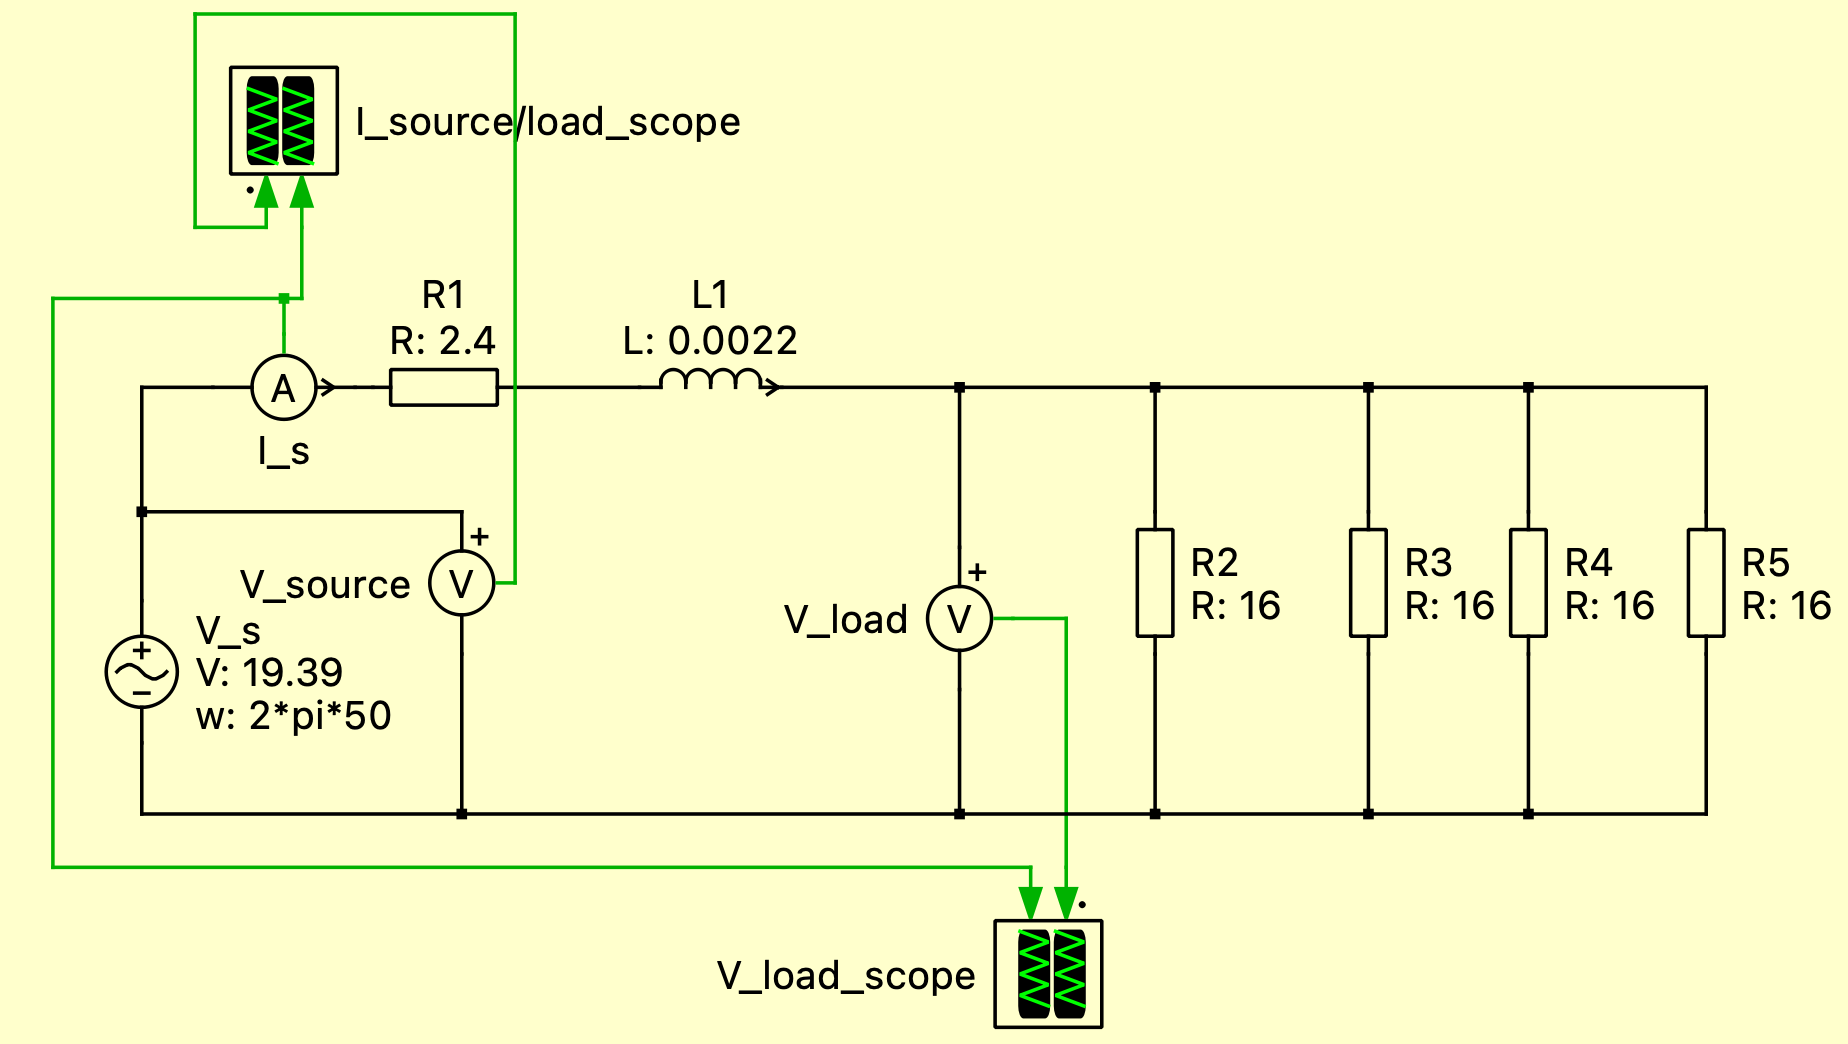
\includegraphics[width=0.5\linewidth]{images/Sim.3.png}
        \caption{Simulation of Circuit Fig \ref{fig:transmission_line_losses_without_transformer}}
        \label{fig:Sim.3}
    \end{figure}
    
    \pagebreak
    \subsection{Estimating Loss in Transmission Line with Transformers}

    \begin{figure}[ht]
        \centering
        \begin{circuitikz}
            % Source and transmission line
            
            \draw (0,4) 
            to[sV, v={$V_s$}] (0,0);
            \draw (0,4) -- (1.5,4);
            \ctikzset{quadpoles/transformer core/height=2.8565};
            \draw (2,2) node[transformer core](T1){};
            \draw (3,4)
            to[R, l={$2.4\Omega$}, *-*] (6,4)
            to[L, l={$2.2mH$}, *-*] (9,4);
            
             % Transformer
            %\draw (0,0) node[transformer core](T1){};
            % adjust it
            %\ctikzset{quadpoles/transformer core/height=2.86};
            \draw (9.7,2) node[transformer core](T2){};
            
            %\node [ocirc] at (T.B1){}; \node [ocirc] at (T.B2){};
            
            % Resistive loads
            \draw (12,4)
            to[R, l={$16\Omega$}, *-*] (12,0);
            \draw (13,4)
            to[R, l={$16\Omega$}, *-*] (13,0);
            \draw (14,4)
            to[R, l={$16\Omega$}, *-*] (14,0);
            \draw (15,4)
            to[R, l={$16\Omega$}, *-*] (15,0);
                
            % Annotations and dashed line
            \draw[->] (0.5,3.8) -- (1.5,3.8) node[midway, anchor=north] {$I_s$};
            \draw[->] (5.5,3.8) -- (6.5,3.8) node[midway, anchor=north] {$I_{\text{Line}}$};
            \draw[->] (10.5,3.8) -- (11.5,3.8) node[midway, anchor=north] {$I_{\text{Load}}$};
            \draw[->] (11.5,2.5) -- (11.5,1.5) node[midway, anchor=east] {$V_{\text{Load}}$};
            \draw[dashed] (11.7,4.5) -- (16,4.5) -- (16,-0.5) -- (11.7,-0.5) -- cycle;
            \draw (0,0) -- (1.5,0);
            \draw (3,0) -- (9,0);
            \draw (10.5,4) -- (15,4);
            \draw (10.5,0) -- (15,0);
            \node at (14,-1) {R Loads};
            \node at (6,3) {Transmission Line};
        \end{circuitikz}
        \caption{Transmission Line losses}
        \label{fig:transmission_line_losses}
    \end{figure}
    
  
    \begin{table}[H]
       \small
       \centering
       \begin{tabular}{l|ccccccr}
       \toprule\toprule
       \text{} & \textbf{$V_{Source} (V)$} & \textbf{$I_{Source} (A)$} & \textbf{$P_{Source} (W)$} & \textbf{$Q_{Source} (var)$} & \textbf{$P.F.\, Source$} \\
       \midrule
       \text{Measurements}&14.1&2.85&40.2&2.80&0.998\\
       \midrule
       \text{Simulations}&12.1&3.00&36.3&3.00&1.00\\
       \toprule\toprule
       \text{} & \textbf{$I_{Line} (A)$} & \textbf{$V_{Load} (V)$} & \textbf{$I_{Load} (A)$} &
       \textbf{$P_{Load} (W)$} \\
       \midrule
       \text{Measurements}&0.222&12.0&2.56&30.8\\
       \midrule
       \text{Simulations}&0.256&12.0&3.00&36.0\\
       \bottomrule 
       \end{tabular}
       \caption{Measurements: Loss in Transmission Line With Transformers}
       \label{Table8_LineLoss_2}
    \end{table}

    To quantify power losses in the system with transformers, we first calculate the line losses as follows:
    \[
    P_{line} = I^2*R_{line} = (0.222A)^2 * 2.4\Omega \approx 0.118W
    \]
    Next, we evaluate the difference in real power between the source and the load to pinpoint where losses occur:
    \[
    P_{X'mer} = P_{Source} - P_{Load} = 40.2W - 30.8W = 9.40W
    \]
    To quantify how much real power loss occurred from the Transformers alone we can get an estimate by subtracting all the Power losses from the $P_{Source}$:
    \[
    P_{Transformers} = P_{Source} - P_{Load} - P_{line} = 40.2W - 30.8W - 0.118W = 9.28W
    \]
    To evaluate the efficiency of power transfer from the source to the load, we use the formula:
    \[
    \text{Efficiency (\%)} = \left( \frac{P_{Load}}{P_{Source}} \right) \times 100 = \left( \frac{30.8W}{40.2W} \right) \times 100\% = 76.6\%
    \]

    Lets Compare these results with the simulation. Note however that ideal transformers are used in the simulation, suggesting near-perfect power transfer and thus a lower simulated $P_{sim.X'mer}$. To model a more realistic scenario, one could include the calculated series and parallel impedances in \hyperref[sub:trans]{section 2} for both transformers. However, given the imprecise resistors used in this study, such a level of detail is unnecessary for the scope of this report given how inaccurate the documentation was on what resistors we used for the measurements.
    
    \begin{align*}
    P_{sim.X'mer} &= P{sim.Source} - P{sim.Load} = U_{sim.Source}*I*P.F._{sim.Source} - U_{sim.Load}*I*P.F._{sim.Load} \\
    P.F._{sim.Source} &= cos( \frac {\delta t}{T}*360 \degree )
    = cos(\frac{0.00}{20ms}*360 \degree ) = cos(0.00 \degree ) = 1.00 \\
    P.F._{sim.Load} &= cos( \frac {\delta t}{T}*360 \degree )
    = cos(\frac{0.00ms}{20ms}*360 \degree ) = cos(0.00 \degree ) = 1.00 \\
    P_{sim.X'mer} &= P{sim.Source} - P{sim.Load} = 12.1V*3.00A*1 - 12.0V*3.00A*1\\
    P_{sim.X'mer} &= 36.3W - 36.0W = 0.03W 
    \end{align*}
    stating that our guess was correct.
    
    \begin{figure}[ht]
        \centering
        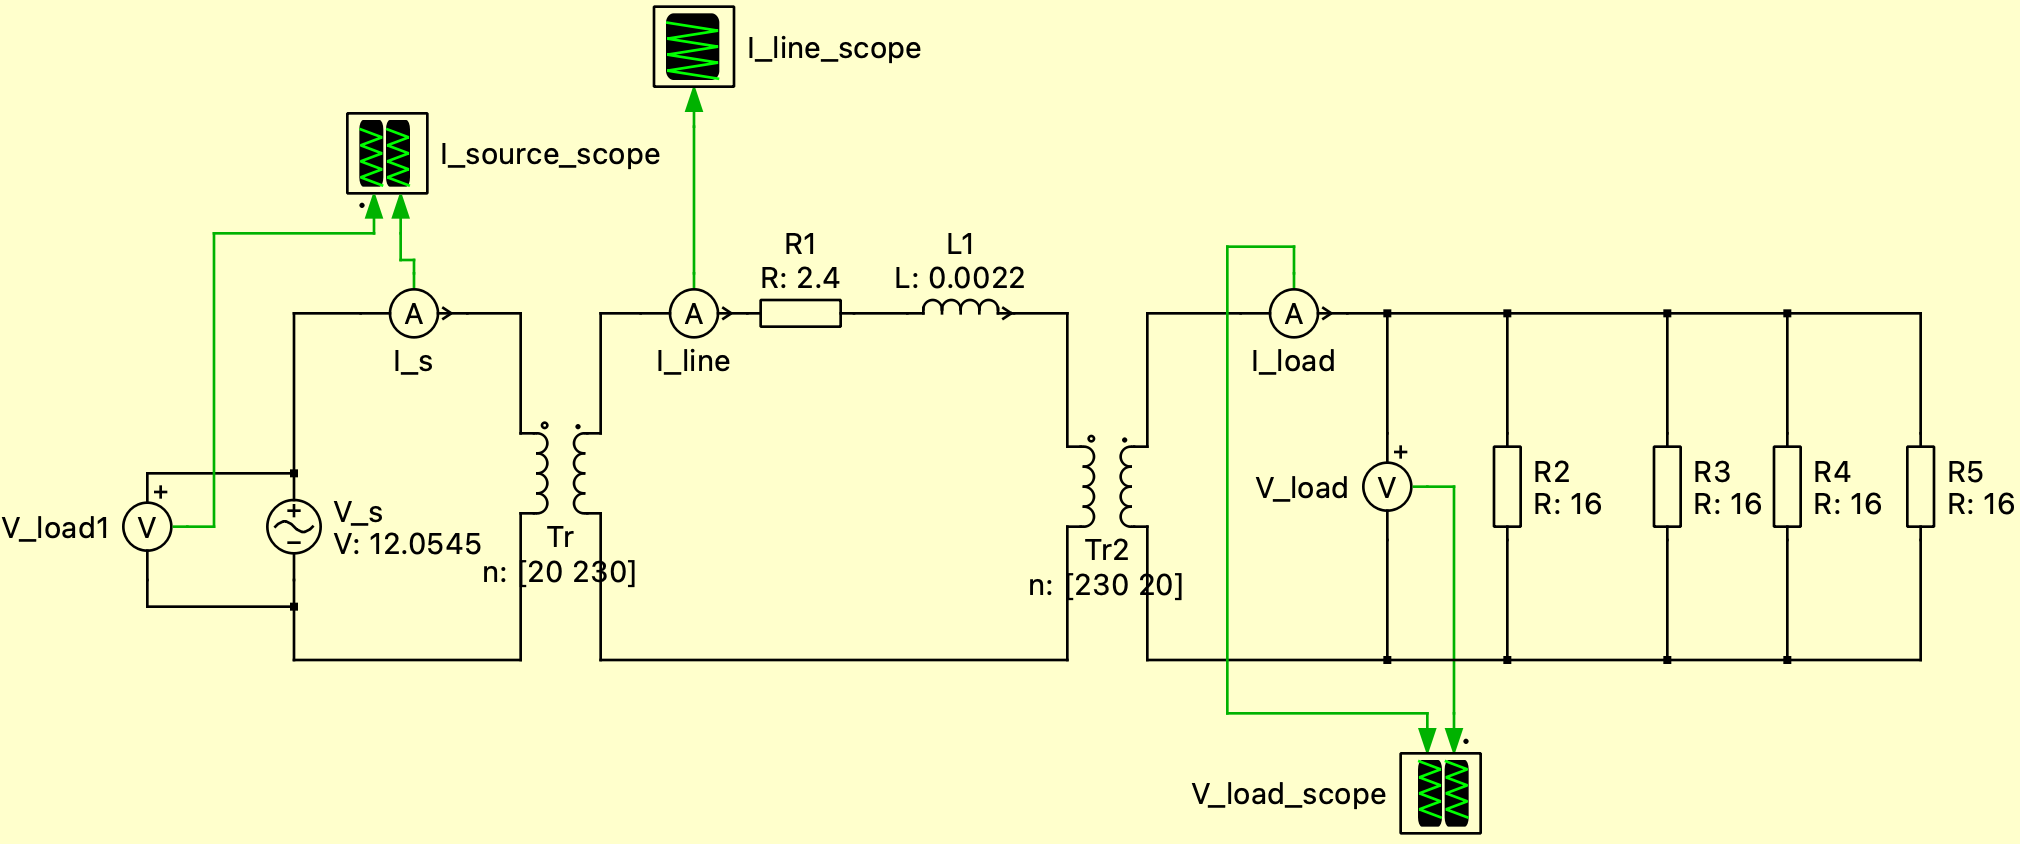
\includegraphics[width=0.65\linewidth]{images/Sim.4.png}
        \caption{Simulation of Circuit Fig \ref{fig:transmission_line_losses}}
        \label{fig:sim.4}
    \end{figure}

\subsection{Comparisson in Efficiency of Power Transferred}

    The calculated line losses and transformer power draw indicate a clear advantage in using transformers. Specifically, the reduction in losses and improvement in efficiency are as follows:
    
    \begin{align*}
    P_{WithoutTransformersX'mer} &= 17.2W \\
    P_{WithTransformersX'mer} &= 9.40W \\
    \Delta P_{X'mer} = 17.2W - 9.40W &= 7.8W\\
    \Delta \text{Efficiency (\%)} = Eff_{WithTransformers} - Eff_{WithoutTransformers} &= 76.6\% - 64.3\% = 12.3\%
    \end{align*}

    Thus, we observe a reduction in losses of 7.8W and an efficiency gain of 12.3\% when using transformers. These findings highlight the effectiveness of transformers in reducing line losses.
    
    To understand why the net efficiency improves despite additional transformer losses, we examine the voltage drop across the transmission line in both scenarios. First, considering Figure \ref{fig:transmission_line_losses_without_transformer} and a power factor of 1, the voltage drop is calculated as:

    \[ 
    V_{Line} = V_{Source} - V_{Load} = 18.7V - 12.01V = 6.69V
    \]
    This corresponds to: 
    \[ 
    \frac{V_{Line}}{V_{Source}} \times 100 =  \frac{6.69V}{18.7V} * 100\% = 35.8\%
    \]
    Now lets calculate it of Figure \ref{fig:transmission_line_losses} which is with the use of transformers:
    \[
    V_{Line} = V_{Source} - V_{Load} = 14.1V - 12.0V = 2.1V
    \]
    which translates to 
    \[ 
    \frac{V_{Line}}{V_{Source}} \times 100 =  \frac{2.1V}{14.1V} * 100\% = 14.9\%
    \] 

    This diminished voltage drop results from the step-up transformer elevating the voltage by a factor of $\frac{230}{20} = 11.5$
    thus reducing the current in the transmission line by the same factor. This, in turn, decreases the associated power losses. The mitigation of these losses by the transformers explains the lower voltage drop and the improved overall system efficiency.
    
\end{homeworkProblem}

\pagebreak

\begin{homeworkProblem}  

    \subsection{Possible Errors and Improvement}\label{subsec:erors} 
    
    In the investigation of electrical power systems, both through experimentation and simulation, a variety of errors can compromise the accuracy of outcomes. These include instrumentation inaccuracies due to the lack of proper calibration of devices like voltmeters. The real-world behavior of components introduces additional errors; for example, parasitic elements in inductors and capacitors can deviate from ideal models. Environmental variables like temperature can also alter material properties, affecting readings. However Human error still remains the most significant source of inaccuracy, stemming from misinterpretation of readings, miss reading of measurements, incorrect setups, and improper component selection. Lastly, simplified models, such as those assuming ideal transformers, may not align with real-world scenarios. To mitigate these issues, calibration of all instruments is essential. Modeling should incorporate non-ideal behaviors of components, and environmental conditions should be controlled or accounted for in data interpretation. Multiple rounds of measurements can statistically minimize human error, and it's crucial to verify the availability and specifications of all components, prior to experimentation.
    
    \subsection{Power Factor Improvement and the use of Transformers}

    Improving the power factor has several advantages in electrical power systems. A more efficient power factor reduces losses, especially in transmission lines, leading to a more efficient power system. This efficiency translates to decreased electricity costs. Additionally, utilities might impose extra charges on consumers with a low power factor. An improved power factor can also enhance the capacity of the electrical system, meaning the current infrastructure can handle more loads without needing upgrades. Moreover, a better power factor can lead to a reduced voltage drop across transmission lines, ensuring equipment operates within their voltage range.
    
    Transformers, on the other hand, are vital in power systems. They allow for the efficient transmission of power over long distances by adjusting the voltage levels. This adjustment reduces current and, consequently, losses, before being stepped down for end-user consumption. The ability of transformers to adjust voltage levels offers flexibility in designing power systems, integrating various energy sources and loads seamlessly. In addition some systems only work in a certain voltage range so having a tool that can efficiently step down/up the voltage is an incredibly useful tool. For those reasons it is unimaginable to think of our electrical infrastructure without the use of transformers.

\end{homeworkProblem}
%
% Non sequential homework problems
%


\end{document}
